\question{Câu 1}

Cho mạch khuếch đại tín hiệu như hình vẽ. Các tụ $C_{1}$, $C_{2}$ và $C_{3}$ có giá trị rất lớn.

\begin{itemize}[label=-]
	\item  Hình 1: Các giá trị $R_{1} = 500\,\textsf{k}\Omega$, $R_{2} = 1.4\,\textsf{M}\Omega$, $R_{S} = 33\,\textsf{k}\Omega$, $R_{D} = 82\,\textsf{k}\Omega$, $V_{DD} = 16\,\textsf{V}$. MOSFET có $K_{n} = 250\,\mu\textsf{A}/\textsf{V}^{2}$, $V_{TN} = 1.2\,\textsf{V}$ và $V_{A} = \infty$. 
	\item  Hình 2: Các giá trị $R_{1} = 2.2\,\textsf{M}\Omega$, $R_{2} = 2.2\,\textsf{M}\Omega$, $R_{S} = 22\,\textsf{k}\Omega$, $R_{D} = 18\,\textsf{k}\Omega$ và $V_{DD} = 20\,\textsf{V}$. FET có $K_{p} = 400\,\mu\textsf{A}/\textsf{V}^{2}$, $V_{TP} = -1.5\,\textsf{V}$ và $V_{A} = \infty$. 
\end{itemize}

\begin{figure}[H]
	\centering
	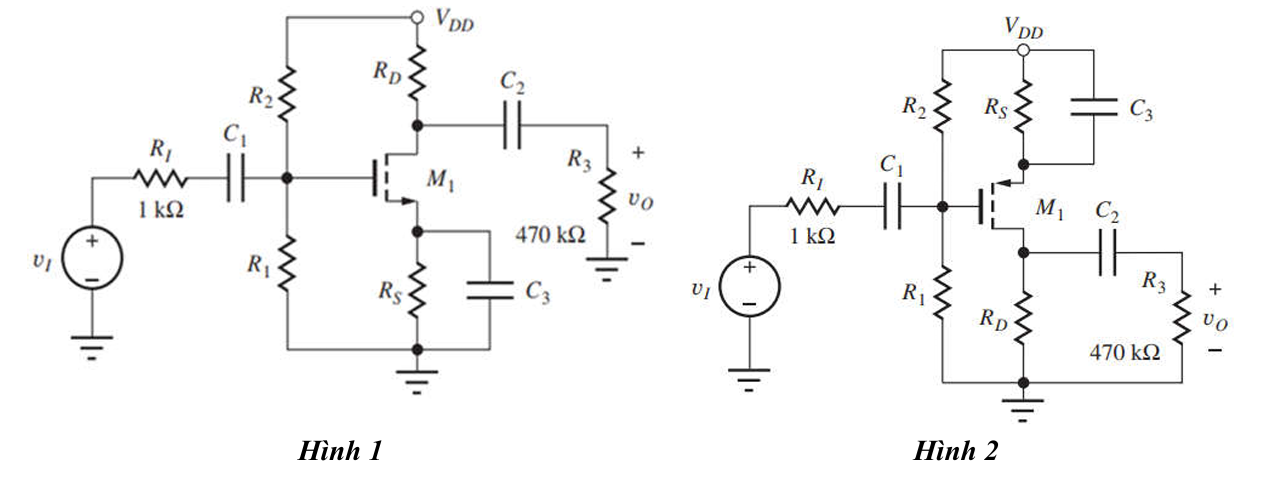
\includegraphics[width=\linewidth]{./my-chapters/my-images/Question1/debai.png}
\end{figure}

\begin{center}
	\textbf{Ở hình 1}
\end{center}

\answer{a1}{Vẽ VTC của mạch và tìm hiểu điểm hoạt động $Q$ của FET.}

\noindent Vẽ VTC của mạch

\begin{itemize}[label=-]
	\item $v_{GS}<V_{TN}=1.2\,\textsf{V}$: MOSFET hoạt động ở trạng thái \textbf{cut-off}  
	\[
	\Rightarrow i_{D}=0 \Rightarrow v_{DS}=V_{DD}=16\,\textsf{V}
	\]
	
	\item $v_{GS}=V_{TN}$: MOSFET hoạt động ở trạng thái \textbf{saturation (bão hoà)}  
	\[
	\Rightarrow i_{D}=\frac{1}{2}\times K_{n}\left(v_{GS}-V_{TN}\right)^{2}
	\]
	\[
	\Rightarrow v_{DS}=V_{DD}-\left(R_{D}+R_{S}\right)\times\frac{1}{2}\times K_{n}\left(v_{GS}-V_{TN}\right)^{2}
	\]
	\[
	\Rightarrow v_{DS}=16-14.375\left(v_{GS}-1.2\right)^{2}
	\]
	
	\item $v_{GS}\geq\left.v_{GS}\right|_{v_{DS}={v_{DS}}_{sat}}$: MOSFET hoạt động ở trạng thái \textbf{triode}  
	\[
	\Rightarrow i_{D}=K_{n}\left[\left(v_{GS}-V_{TN}\right)v_{DS}-\frac{{v_{DS}}^{2}}{2}\right]
	\]
	\[
	\Rightarrow v_{DS}=V_{DD}-\left(R_{D}+R_{S}\right)\times K_{n}\left[\left(v_{GS}-V_{TN}\right)v_{DS}-\frac{{v_{DS}}^{2}}{2}\right]
	\]
	\[
	v_{DS}={v_{DS}}_{sat}=v_{GS}-V_{TN}
	\]
	\[
	\Rightarrow v_{GS}=V_{TN}+\frac{\sqrt{2V_{DD}\left(R_{D}+R_{S}\right)\times K_{n}}-1}{\left(R_{D}+R_{S}\right)\times K_{n}}
	\]
	\[
	\Rightarrow v_{GS}=2.22\,\textsf{V}
	\]
	\[
	\Rightarrow i_{D}=0.13\,\textsf{mA}
	\]
	
	\item \textbf{Điểm chuyển:}  
	\[
	V_{i}=V_{GS}+V_{S}=V_{GS}+I_{D}R_{S}=6.51\,\textsf{V}
	\]
\end{itemize}

\begin{figure}[H]
	\centering
	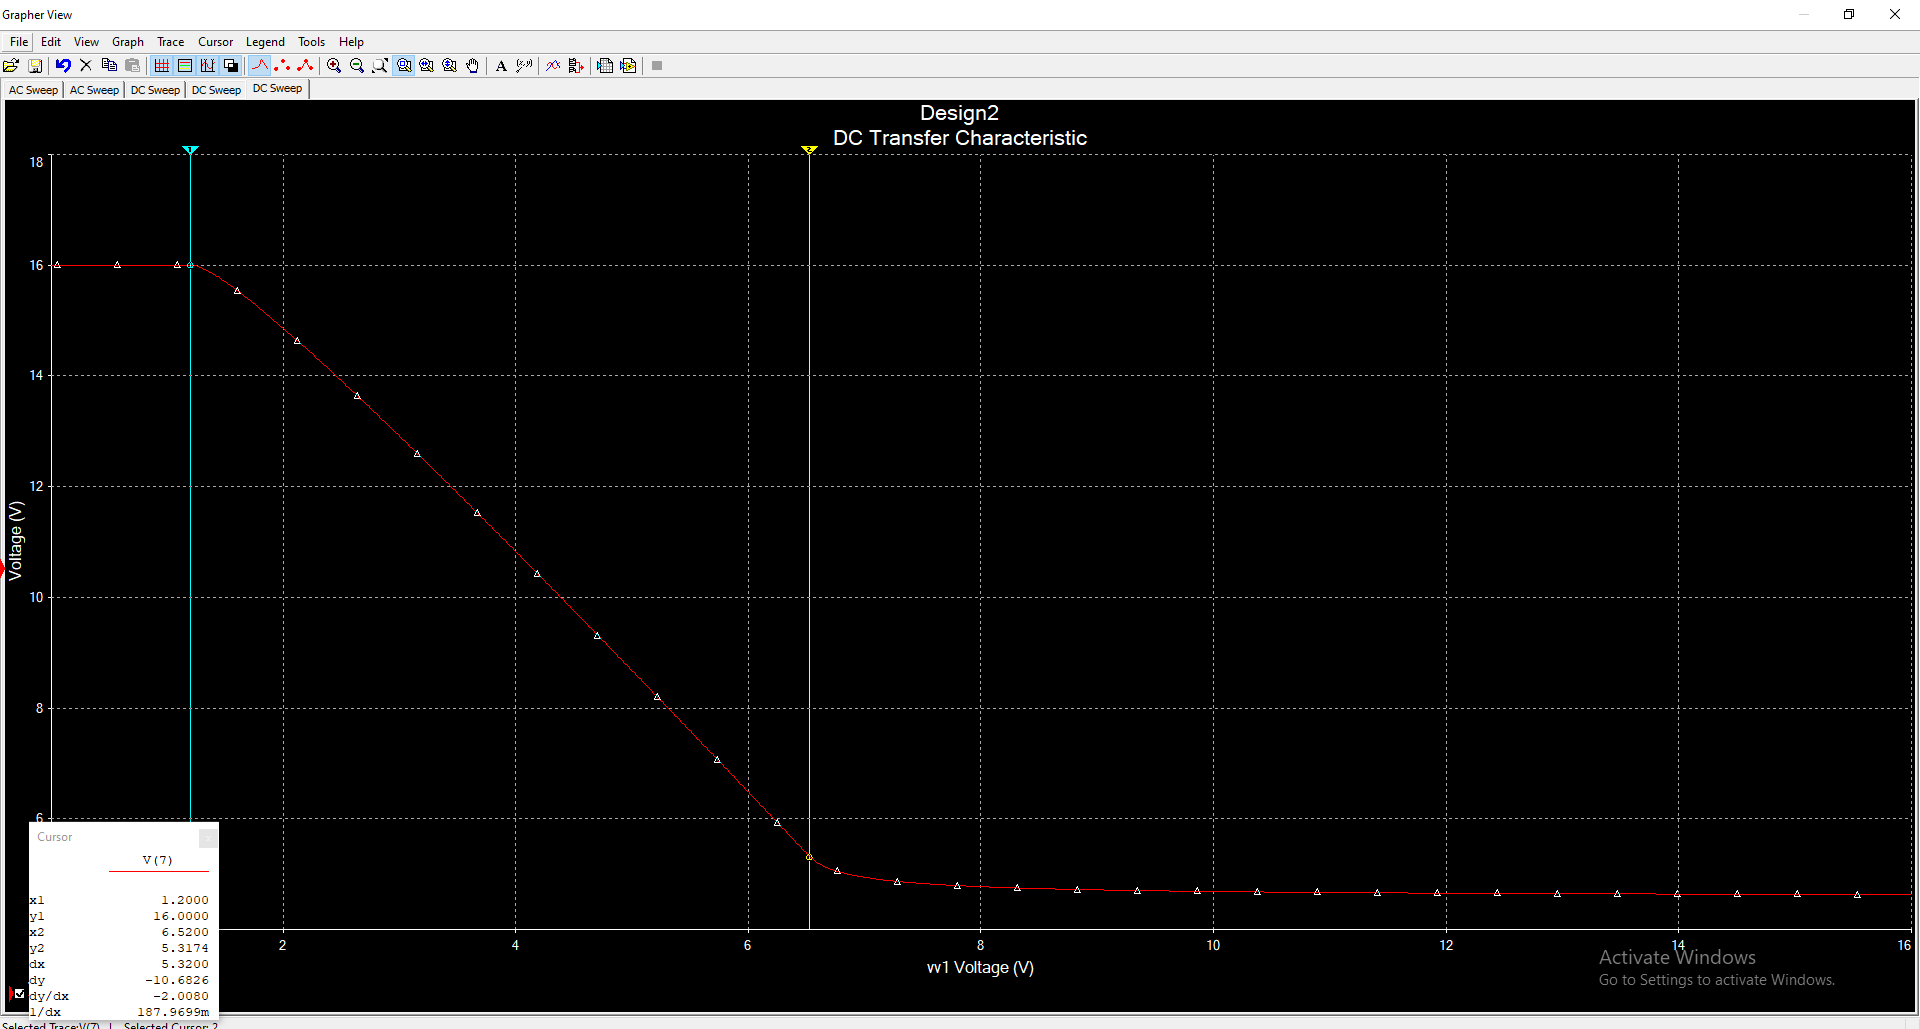
\includegraphics[width=\linewidth]{./my-chapters/my-images/Question1/a1_VTC.png}
	\caption{VTC của mạch ở hình 1.}
\end{figure}

\noindent Tìm điểm hoạt động Q:

%\[
%V_{G}=V_{DD} \frac{R_{1}}{R_{1}+R_{2}}=16\times\frac{500}{500+1400}=4.21\,\textsf{V}
%\]
%\[
%V_{DS}=V_{DD}-\left(R_{D}+R_{S}\right)\times\frac{1}{2}\times K_{n}\left(V_{GS}-V_{TN}\right)^{2}
%\]
%\[
%V_{S}=I_{D}  R_{S}
%\]
%\[
%\begin{aligned}
%	\Rightarrow\; V_{GS} &= V_{DD}\,\frac{R_{1}}{R_{1}+R_{2}}
%	- \frac{1}{2} K_{n} (V_{GS}-V_{TN})^{2} R_{S} \\[6pt]
%	&= 16\,\frac{500}{500+1400}
%	- \frac{1}{2}\times 0.25 \times 33 \times (V_{GS}-1.2)^{2} \\[6pt]
%	&= 1.94\,\textsf{V}
%\end{aligned}
%\]
%
%\[
%V_{DS}=V_{DD}-\left(R_{D}+R_{S}\right)\times\frac{1}{2}\times K_{n}\left(V_{GS}-V_{TN}\right)^{2}
%\]
%\[
%\Rightarrow V_{DS}=16-115\times0.5\times0.25\times\left(1.94-1.2\right)=8.13\,\textsf{V}
%\]
%\[
%I_{DQ}=\frac{1}{2}K_{n}\left(V_{GS}-V_{TN}\right)^{2}
%\]
%\[
%\Rightarrow I_{DQ}=\frac{1}{2}\times0.25\times\left(1.94-1.2\right)^{2}=0.068\,\textsf{mA}
%\]
%
%Vậy điểm làm việc $Q$ là: \finalresult{\left(I_{DQ},V_{DS}\right)=\left(0.068\,\textsf{mA},\,8.13\,\textsf{V}\right)}.

\[
V_{G}=V_{DD}\,\frac{R_{1}}{R_{1}+R_{2}}=16\times\frac{500}{500+1400}=4.21\,\textsf{V}
\]

\[
V_{DS}=V_{DD}-\left(R_{D}+R_{S}\right)\times\frac{1}{2}\times K_{n}\left(V_{GS}-V_{TN}\right)^{2}
\]

\[
V_{S}=I_{D}R_{S}
\]

\[
\begin{aligned}
	\Rightarrow\; V_{GS} &= V_{DD}\,\frac{R_{1}}{R_{1}+R_{2}}
	- \frac{1}{2}K_{n}(V_{GS}-V_{TN})^{2}R_{S} \\[6pt]
	&= 16\,\frac{500}{500+1400}
	- \frac{1}{2}\times0.25\times33\times(V_{GS}-1.2)^{2} \\[6pt]
	&= 1.94\,\textsf{V}
\end{aligned}
\]

\[
V_{DS}=V_{DD}-\left(R_{D}+R_{S}\right)\times\frac{1}{2}\times K_{n}\left(V_{GS}-V_{TN}\right)^{2}
\]
\[
\Rightarrow V_{DS}=16-115\times0.5\times0.25\times(1.94-1.2)^{2}=8.13\,\textsf{V}
\]

\[
I_{DQ}=\frac{1}{2}K_{n}\left(V_{GS}-V_{TN}\right)^{2}
\]
\[
\Rightarrow I_{DQ}=\frac{1}{2}\times0.25\times(1.94-1.2)^{2}=0.068\,\textsf{mA}
\]

Vậy điểm làm việc $Q$ là: \finalresult{\left(I_{DQ},V_{DS}\right)=\left(0.068\,\textsf{mA},\,8.13\,\textsf{V}\right)}.

Kiểm chứng kết quả

\begin{figure}[H]
	\centering
	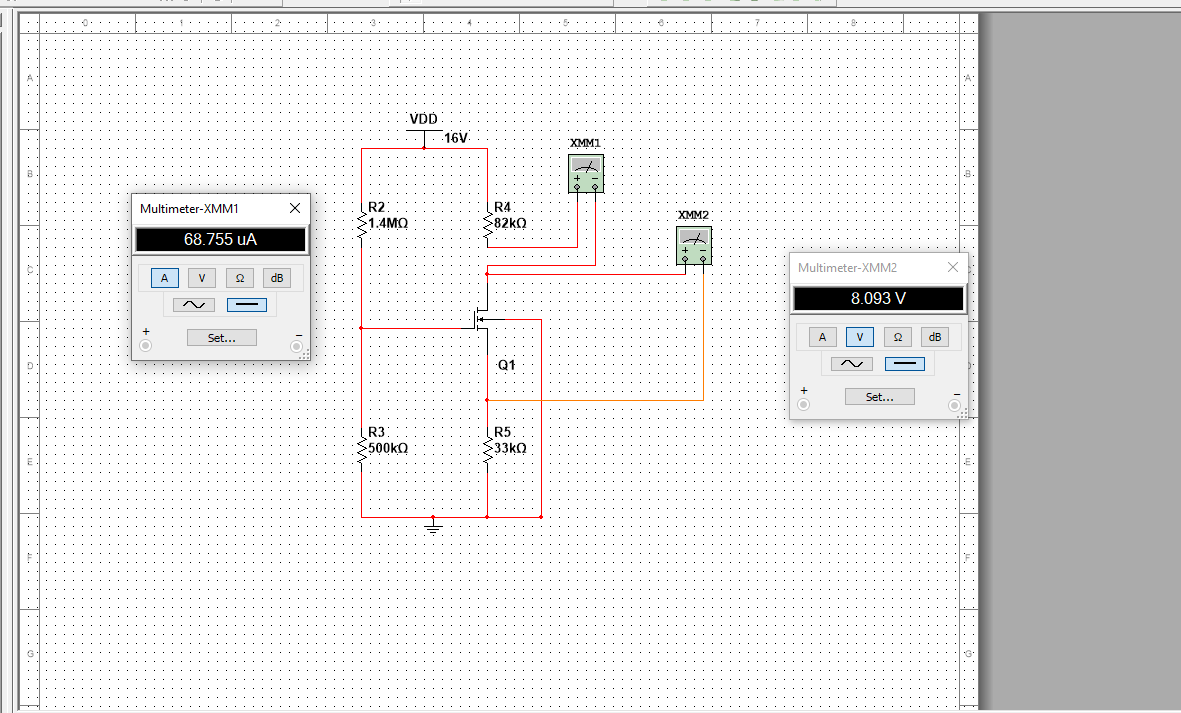
\includegraphics[width=\linewidth]{./my-chapters/my-images/Question1/Câu 1 Hình 1 a - Điểm Q.png}
\end{figure}

\answer{b1}{Đặt $v_{1} = V_{m} \sin \left( \omega t\right)$ vào mạch. Tìm $A_{vo}$, $G_v$, $R_i$, $R_o$ của mạch.}

\[
R_{i}=R_{1}\,//\,R_{2}=\frac{500\times1400}{500+1400}=368.42\,\textsf{k}\Omega
\]
$\Rightarrow$ \finalresult{R_{i} = 368.42\,\textsf{k}\Omega}.

\[
R_{o}=R_{D}=82\,\textsf{k}\Omega
\]
$\Rightarrow$ \finalresult{R_{o}=82\,\textsf{k}\Omega}.
\[
g_{m}=\frac{2I_{DQ}}{V_{GSQ}-V_{TN}}=0.184\,\textsf{mS}
\]
\[
A_{vo}=-g_{m}R_{D}=-15.088\,\textsf{V/V}
\]
$\Rightarrow$ \finalresult{A_{vo} = 15.088\,\textsf{V/V}}.
\[
A_{v}=A_{vo}\times\frac{R_{L}}{R_{o}+R_{L}}=-15.088\times\frac{470}{82+470}=-12.85\,\textsf{V/V}
\]
$\Rightarrow$ \finalresult{A_{v} = -12.85\,\textsf{V/V}}.
\[
G_{v}=A_{vo}\times\frac{R_{L}}{R_{o}+R_{L}}\times\frac{R_{i}}{R_{o}+R_{i}}=-15.088\times\frac{470}{82+470}\times\frac{368.42}{1+368.42}=-12.81\,\textsf{V/V}
\]
$\Rightarrow$ \finalresult{G_{v}= -12.81\,\textsf{V/V}}.

Kiểm tra kết quả

\begin{figure}[H]
	\centering
	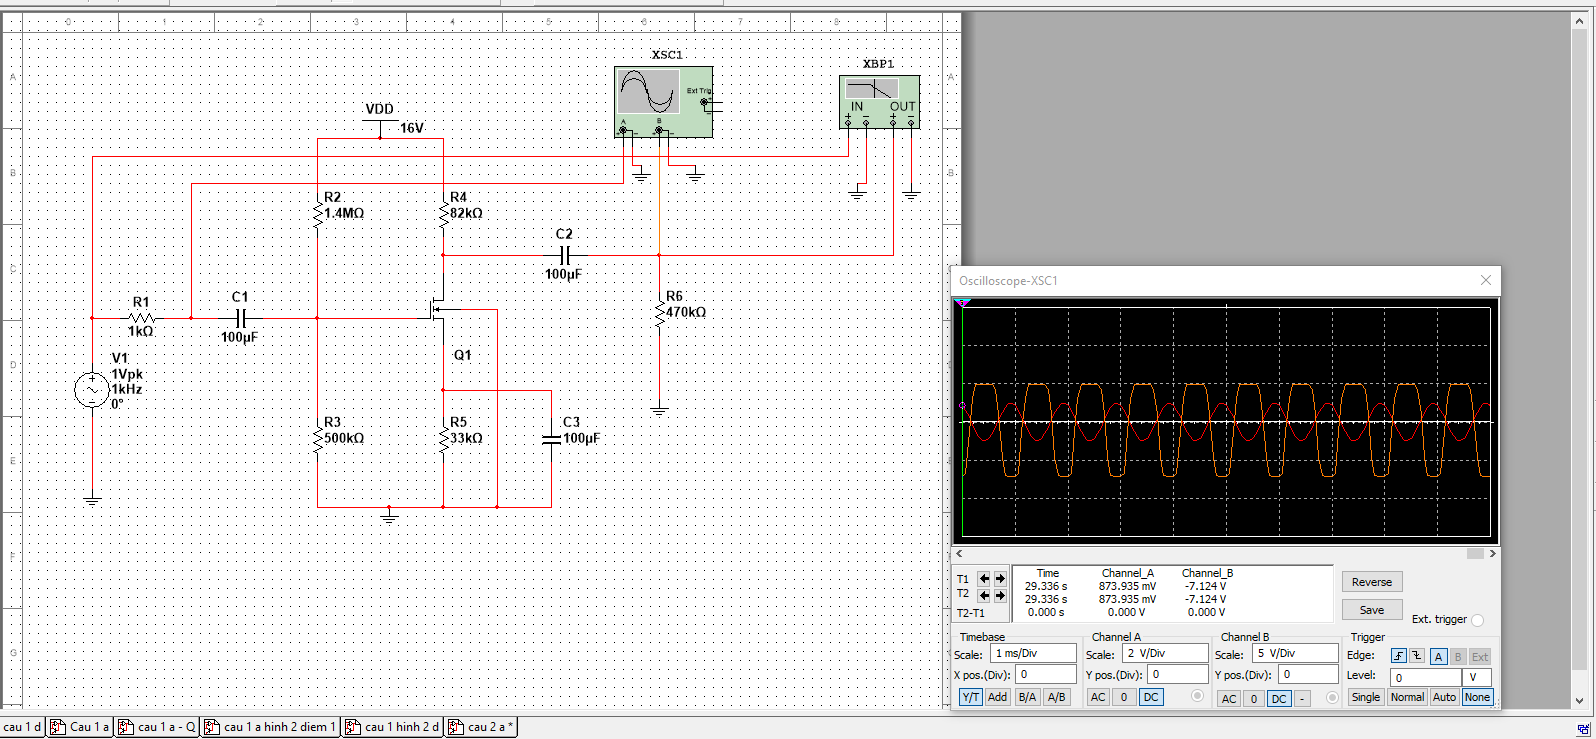
\includegraphics[width=\linewidth]{./my-chapters/my-images/Question1/Câu 1 Hình 1 b - Sóng.png}
	\caption{Dạng sóng ngõ vào và ngõ ra của mạch.}
\end{figure}

\begin{figure}[H]
	\centering
	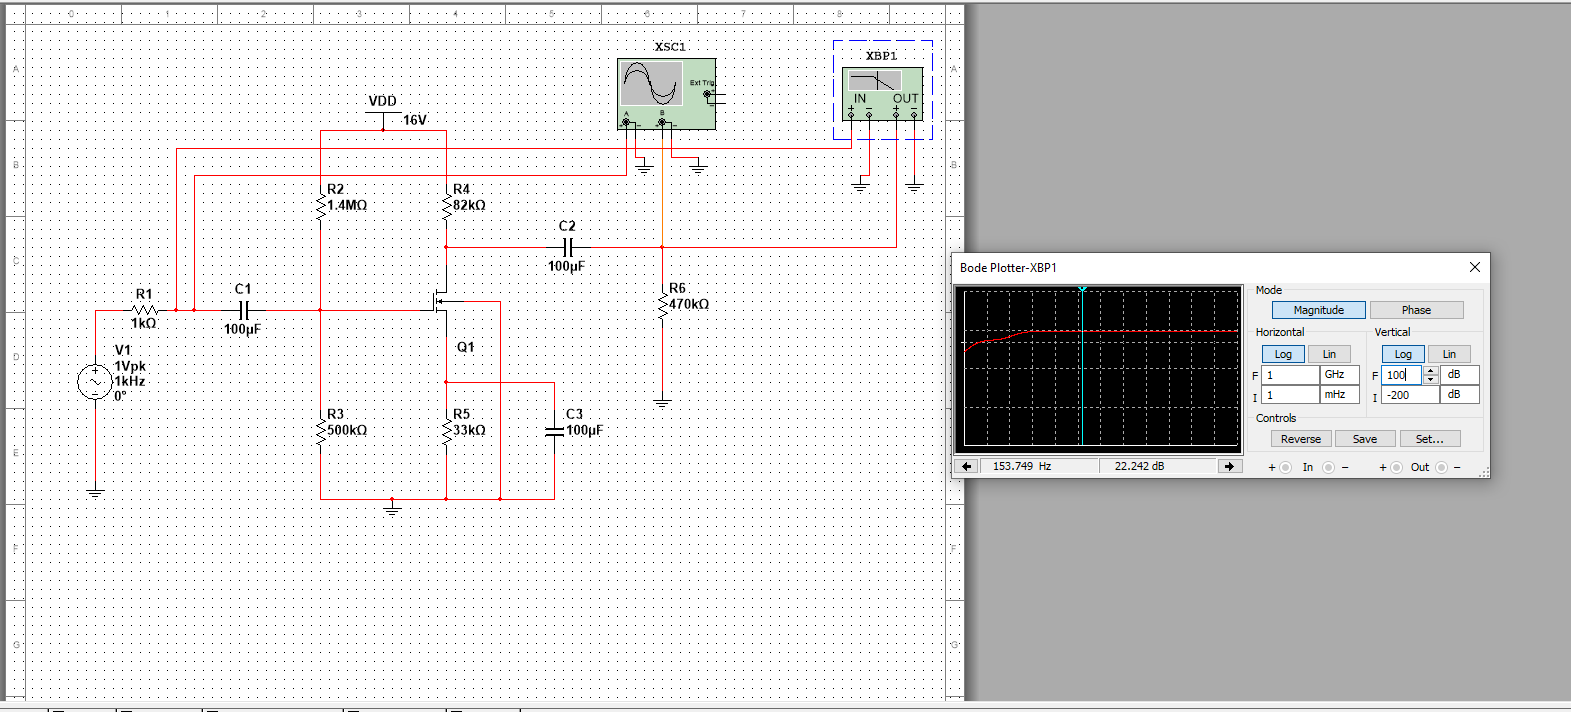
\includegraphics[width=\linewidth]{./my-chapters/my-images/Question1/Câu 1 Hình 1 b - Av.png}
	\caption{Đo $A_{v} = 22.242\,dB \approx 12.9449$.}
\end{figure}

\begin{figure}[H]
	\centering
	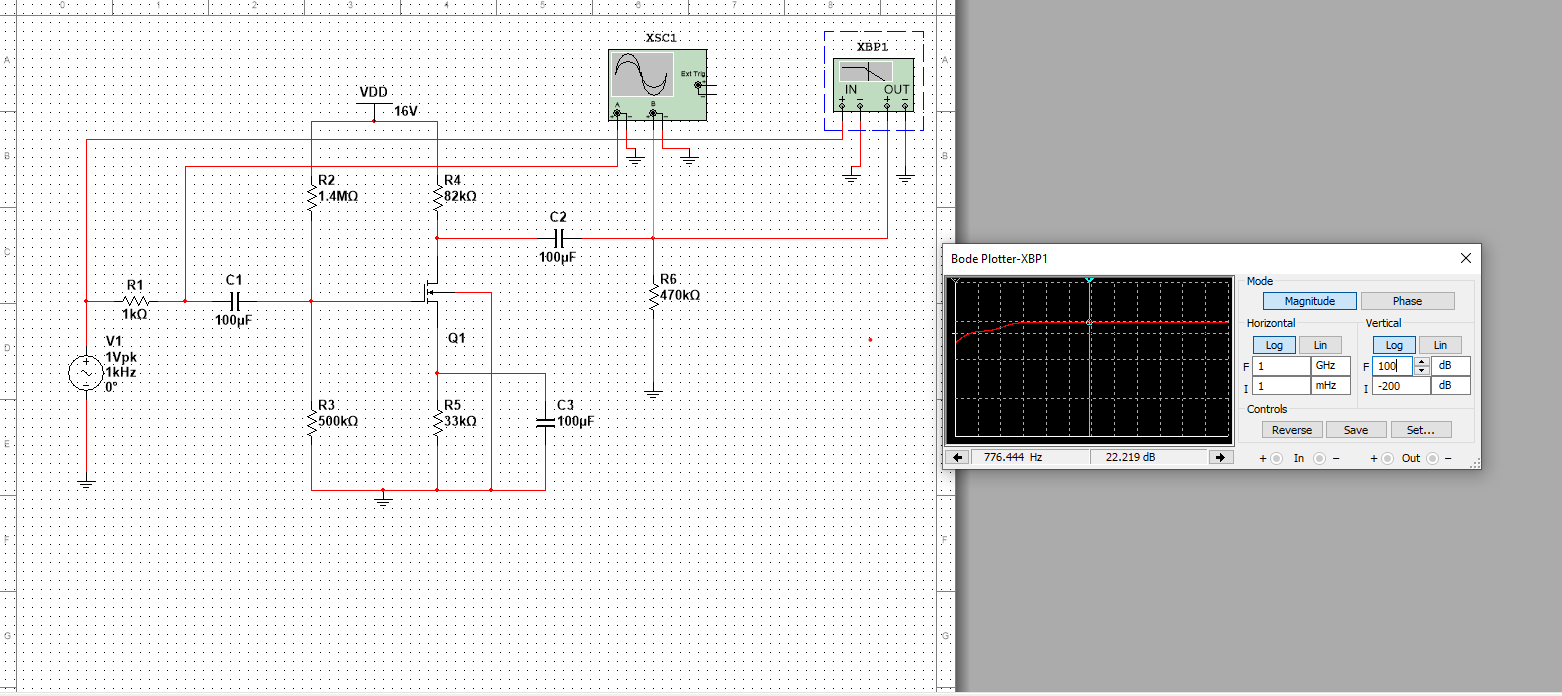
\includegraphics[width=\linewidth]{./my-chapters/my-images/Question1/Câu 1 Hình 1 b - Gv.png}
	\caption{Đo $G_{v} = 22.219\, dB \approx 12.9107$.}
\end{figure}
\answer{c1}{Tìm biên độ lớn nhất của $V_{m}$ để sóng ngõ ra không méo dạng.}
%Từ VTC, ta nhận thấy:
%\[
%{a_{v_{ds}}}_{\text{Max}}=8.13-1.02=7.11\,\textsf{V}
%\Rightarrow {a_{v_{gs}}}_{\text{Max}}=\frac{{a_{v_{ds}}}_{\text{Max}}}{\left|A_{v}\right|}=\frac{7.11}{12.85}=0.55\,\textsf{V}
%\]

Xét điểm $Q$ là: $\left( I_{DQ}\textsf{, } V_{DS}\right) = \left( 0.068\,\textsf{A, } 8.13\,\textsf{V}\right)$
\[ V_{DS} = V_{DD} - \left( R_{D} + R_{S} \right) I_{DQ}\]
\[ \Rightarrow V_{DS} = 16 - 115\,\textsf{k}\times I_{DQ}\]
\[ \tan (\alpha) = \dfrac{1}{R_{D} // R_{3}} = \dfrac{1}{70\,\textsf{k}}\]
\[ \Rightarrow V_{o_{max}} = \dfrac{I_{DQ}}{\tan(\alpha)} = 4.76\,\textsf{V}\]
$\Rightarrow$ \finalresult{V_{sig_{max}} = \dfrac{V_{o_{max}}}{G_{v}\bigg|_{f=776\,\textsf{Hz}} = 0.37\,\textsf{V}}}.

\begin{figure}[H]
	\centering
	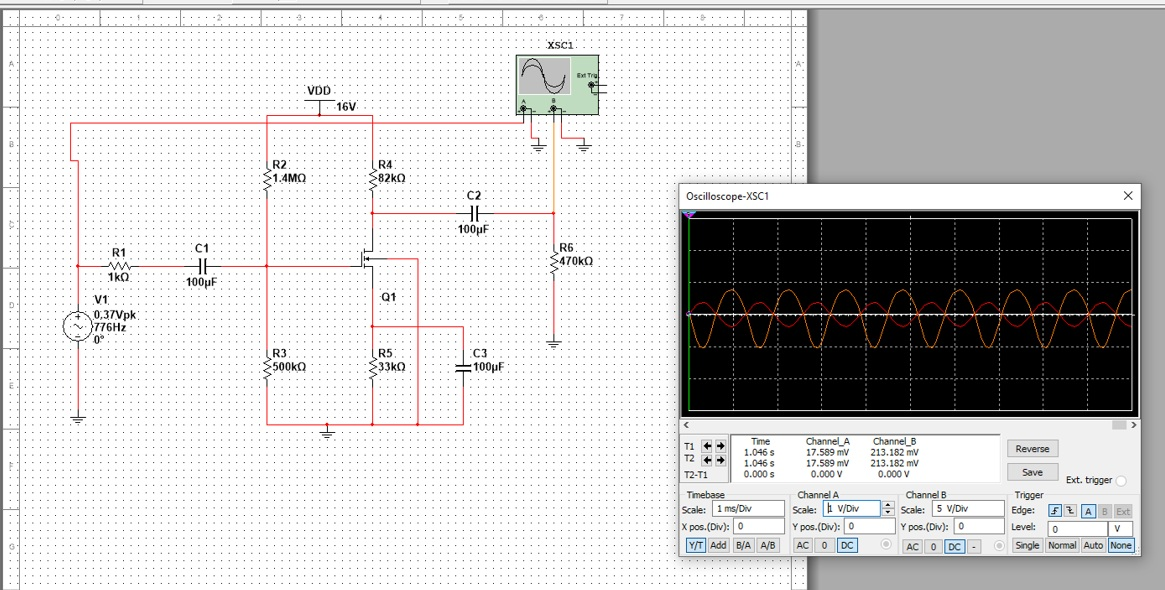
\includegraphics[width=\linewidth]{./my-chapters/my-images/Question1/c_1.jpg}
	\caption{Ngõ ra chưa bị méo dạng.}
\end{figure}
\begin{figure}[H]
	\centering
	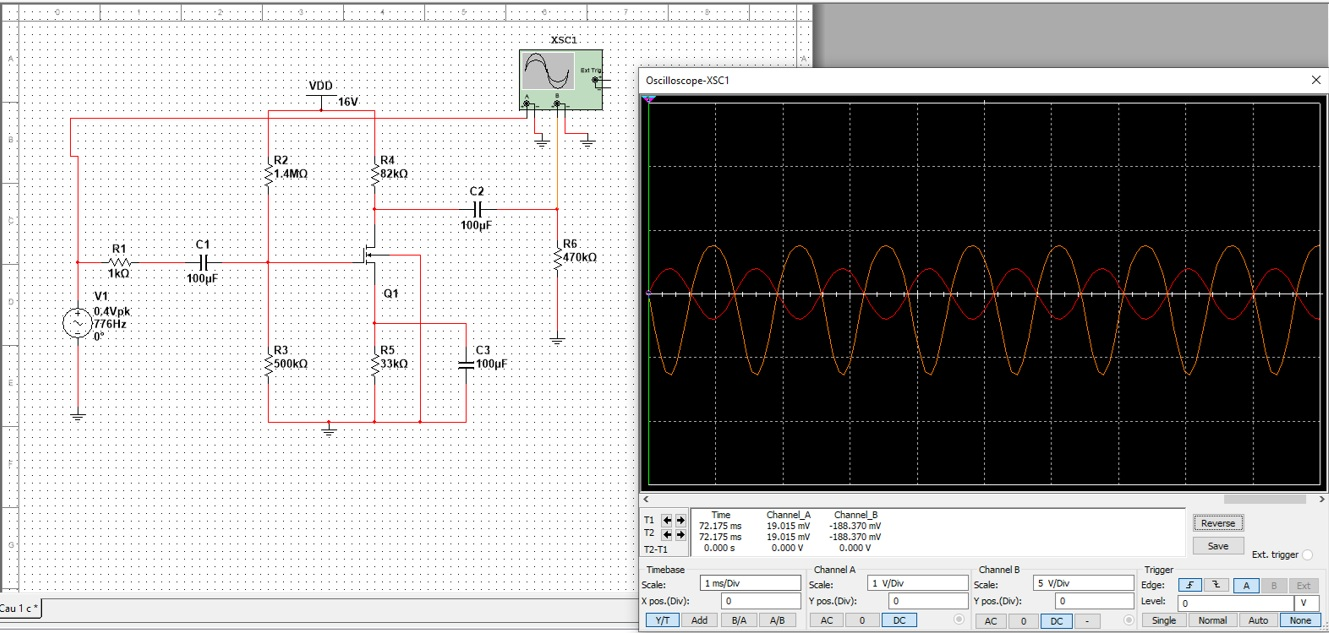
\includegraphics[width=\linewidth]{./my-chapters/my-images/Question1/c_2.jpg}
	\caption{Ngõ ra bị méo dạng.}
\end{figure}

\answer{d1}{Lựa chọn các tụ $C_{1}$, $C_{2}$ và $C_{3}$ để mạch có $f_{L}=100\,\textsf{Hz}$.}

\begin{itemize}[label=-]
	\item Xét ảnh hưởng tụ $C_{1}$: 
	\[
	R_{C_{1}}=R_{1}+R_{in}
	\Longrightarrow \omega_{p_{1}}=\frac{1}{C_{1}(R_{1}+R_{in})}
	\]
	
	\item Xét ảnh hưởng tụ $C_{2}$: 
	\[
	R_{C_{2}}=R_{3}+R_{D}
	\Longrightarrow \omega_{p_{2}}=\frac{1}{C_{2}(R_{3}+R_{D})}
	\]
	
	\item Xét ảnh hưởng tụ $C_{3}$: 
	\[
	R_{C_{3}}=R_{3}\,||\,\frac{1}{g_{m}}
	\Longrightarrow \omega_{p_{3}}=\frac{1}{C_{3}\left(R_{3}\,||\,\frac{1}{g_{m}}\right)}
	\]
\end{itemize}

Theo phương pháp \textbf{cực tần số trội (dominant pole)}, chọn $C_{1}$ làm cực trội có giá trị $100\,\textsf{Hz}$, 
$C_{2}$ và $C_{3}$ tạo ra các cực ở tần số $10\,\textsf{Hz}$.  
Như vậy, tần số cắt của mạch là:
\[
f_{L}=\sqrt{f_{C_{1}}^{2}+f_{C_{2}}^{2}+f_{C_{3}}^{2}}
\]

\textbf{Lựa chọn các tụ $C_{1}$, $C_{2}$, $C_{3}$:}
\[
C_{1}=\frac{1}{2\pi\times100\times\left(1\,\textsf{k}+368.42\,\textsf{k}\right)}=4.31\,\textsf{nF}
\]
\[
C_{2}=\frac{1}{2\pi\times10\times(470\,\textsf{k}+82\,\textsf{k})}=28.8\,\textsf{nF}
\]
\[
C_{3}=\frac{1}{2\pi\times10\times\left(33\,\textsf{k}\,||\,\frac{1}{0.184\,\textsf{mS}}\right)}=3.41\,\mu\textsf{F}
\]

$\Rightarrow$ \finalresult{C_{1} = 4.31\,\textsf{nF}} and \finalresult{C_{2} = 28.8\,\textsf{nF}} and \finalresult{C_{3} = 3.41\,\mu\textsf{F}}.

\begin{figure}[H]
	\centering
	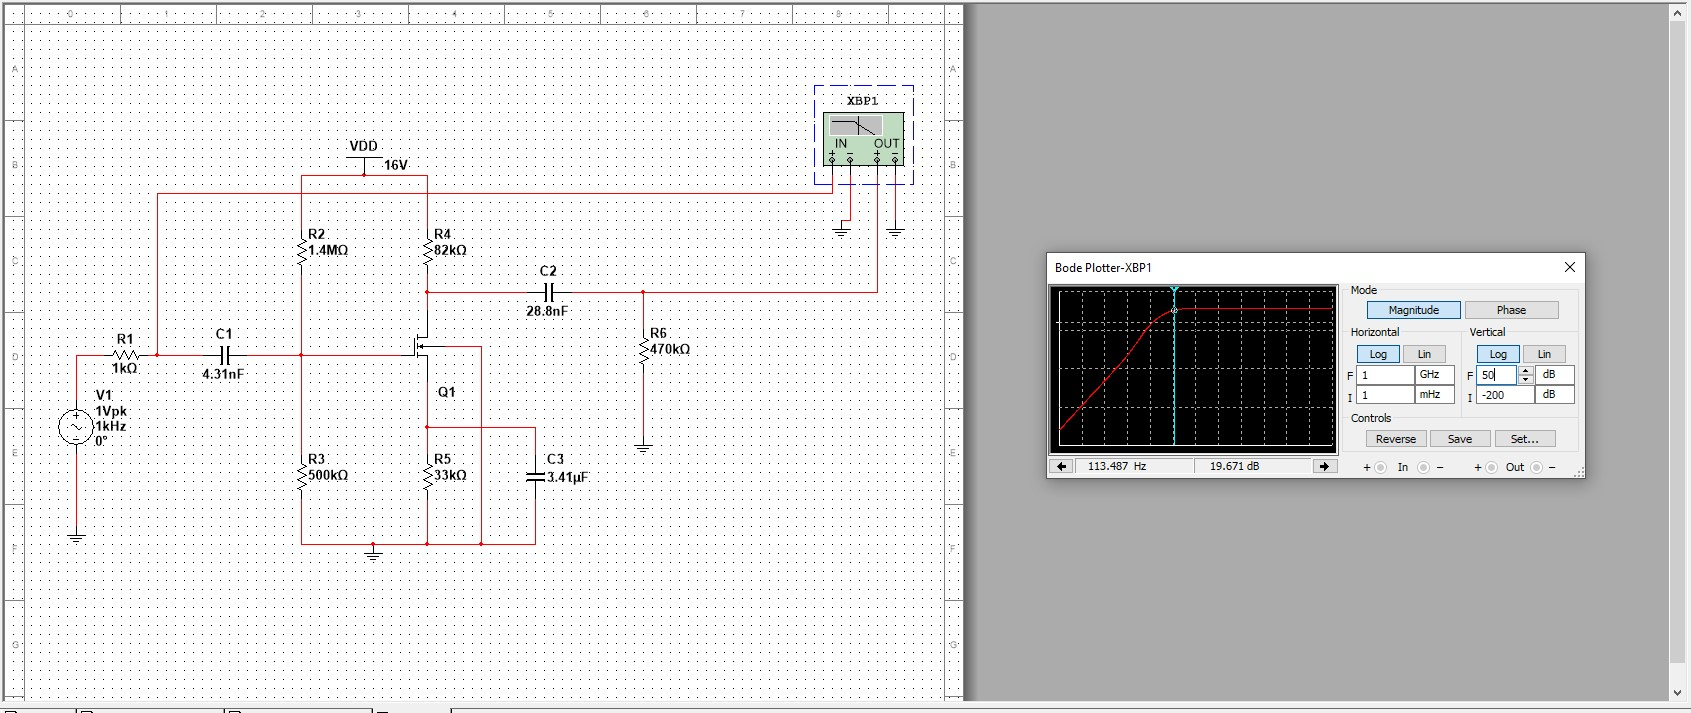
\includegraphics[width=\linewidth]{./my-chapters/my-images/Question1/Câu 1 Hình 1 d.jpg}
\end{figure}

\begin{figure}[H]
	\centering
	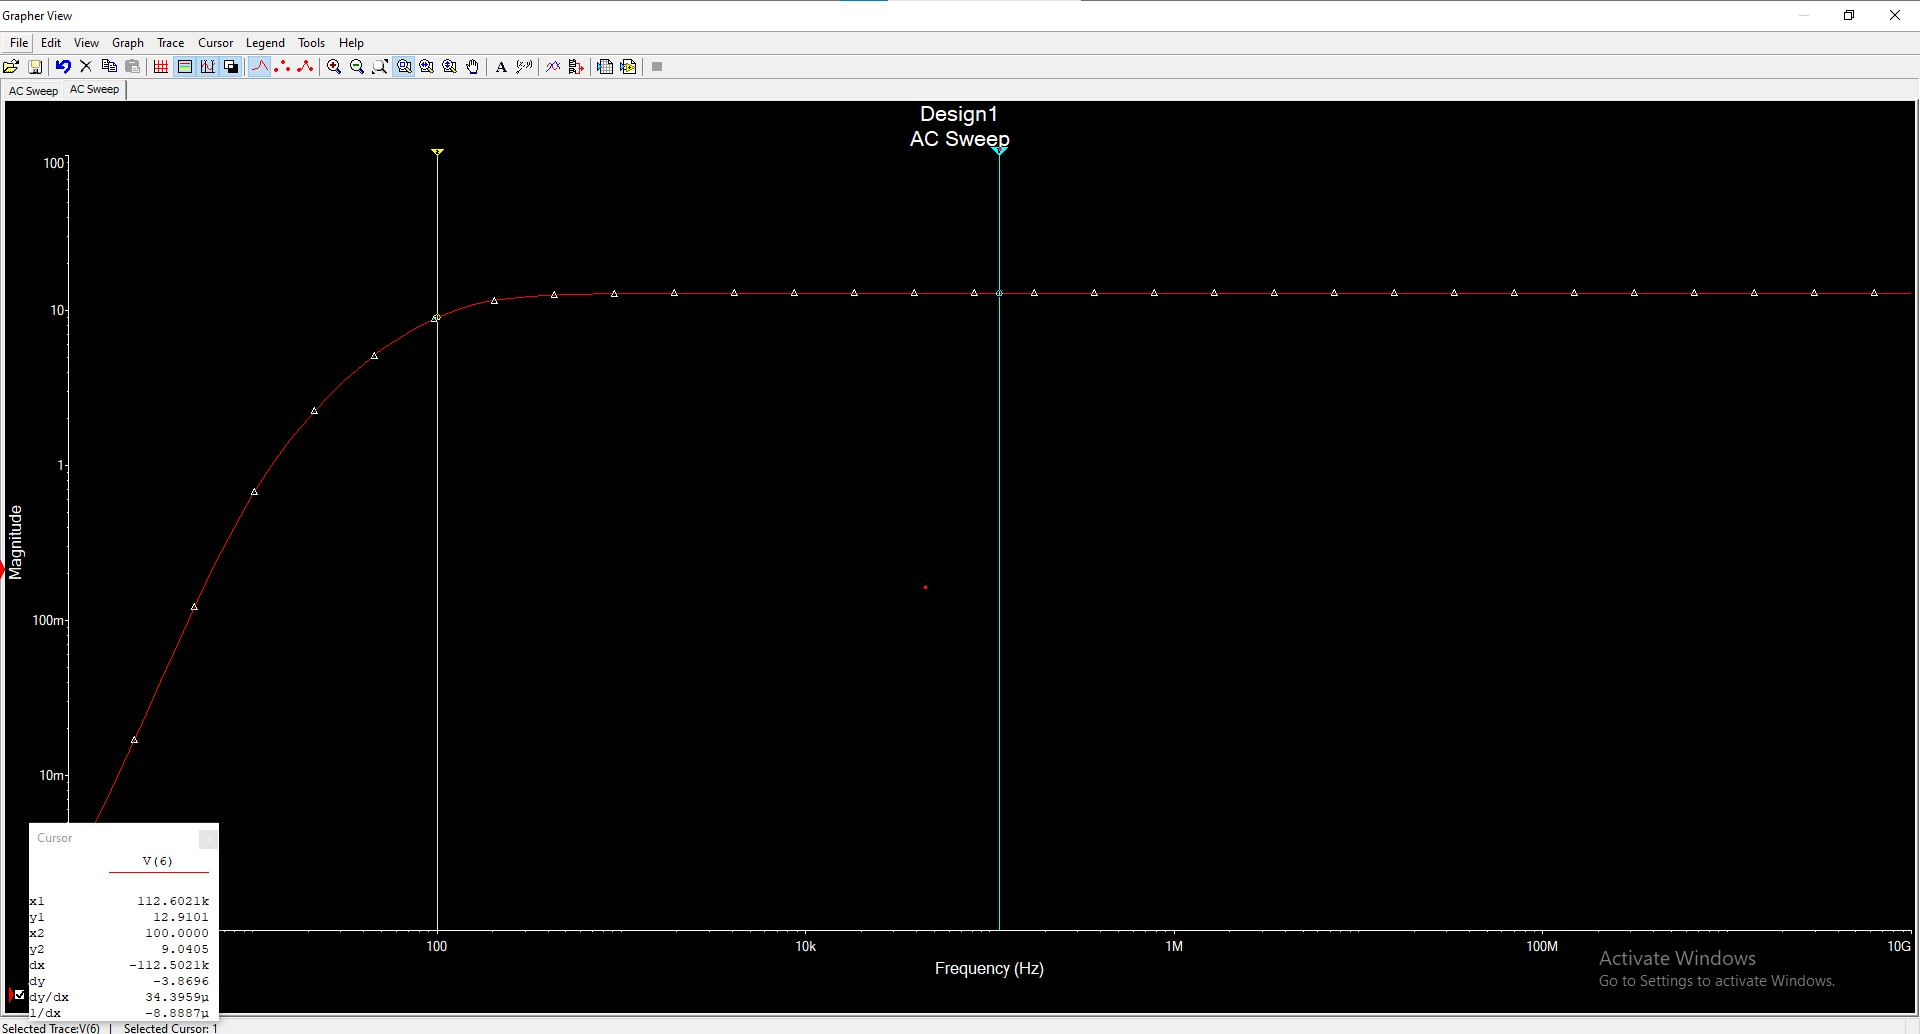
\includegraphics[width=\linewidth]{./my-chapters/my-images/Question1/Câu 1 Hình 1 d - AC sweep.jpg}
\end{figure}

\begin{center}
	\textbf{Ở hình 2}
\end{center}

\answer{a2}{Vẽ VTC của mạch và tìm điểm hoạt động $Q$ của FET.}

\noindent Vẽ VTC của mạch

\begin{itemize}[label=-]
	\item $v_{GS}<V_{TP}$: MOSFET hoạt động ở trạng thái \textbf{cut-off}
	\[
	\Rightarrow i_{D}=0 \Rightarrow v_{DS}=V_{DD}=20\,\textsf{V}
	\]
	
	\item $v_{GS}>V_{TP}$: MOSFET hoạt động ở trạng thái \textbf{saturation (bão hoà)}
	\[
	\Rightarrow i_{D}=\frac{1}{2}\times K_{p}\left(v_{GS}-V_{TP}\right)^{2}
	\]
	\[
	\Rightarrow v_{DS}=V_{DD}-\left(R_{D}+R_{S}\right)\times\frac{1}{2}\times K_{p}\left(v_{GS}-V_{TP}\right)^{2}
	\]
	\[
	\Rightarrow v_{DS}=20-8\left(v_{GS}-1.2\right)^{2}
	\]
	
	\item $v_{GS}\geq \left.v_{GS}\right|_{v_{DS}={v_{DS}}_{sat}}$: MOSFET hoạt động ở trạng thái \textbf{triode}
	\[
	\Rightarrow i_{D}=K_{p}\left[\left(v_{GS}-V_{TP}\right)v_{DS}-\frac{{v_{DS}}^{2}}{2}\right]
	\]
	\[
	\Rightarrow v_{DS}=V_{DD}-\left(R_{D}+R_{S}\right)\times K_{p}\left[\left(v_{GS}-V_{TP}\right)v_{DS}-\frac{{v_{DS}}^{2}}{2}\right]
	\]
	\[
	v_{DS}={v_{DS}}_{sat}=v_{GS}-V_{TP}
	\]
	\[
	\Rightarrow v_{GS}=V_{TP}+\frac{\sqrt{2V_{DD}\left(R_{D}+R_{S}\right)\times K_{p}}-1}{\left(R_{D}+R_{S}\right)\times K_{p}}
	\]
	\[
	\Rightarrow v_{GS}=-3.01\,\textsf{V}
	\]
\end{itemize}

\begin{figure}[H]
	\centering
	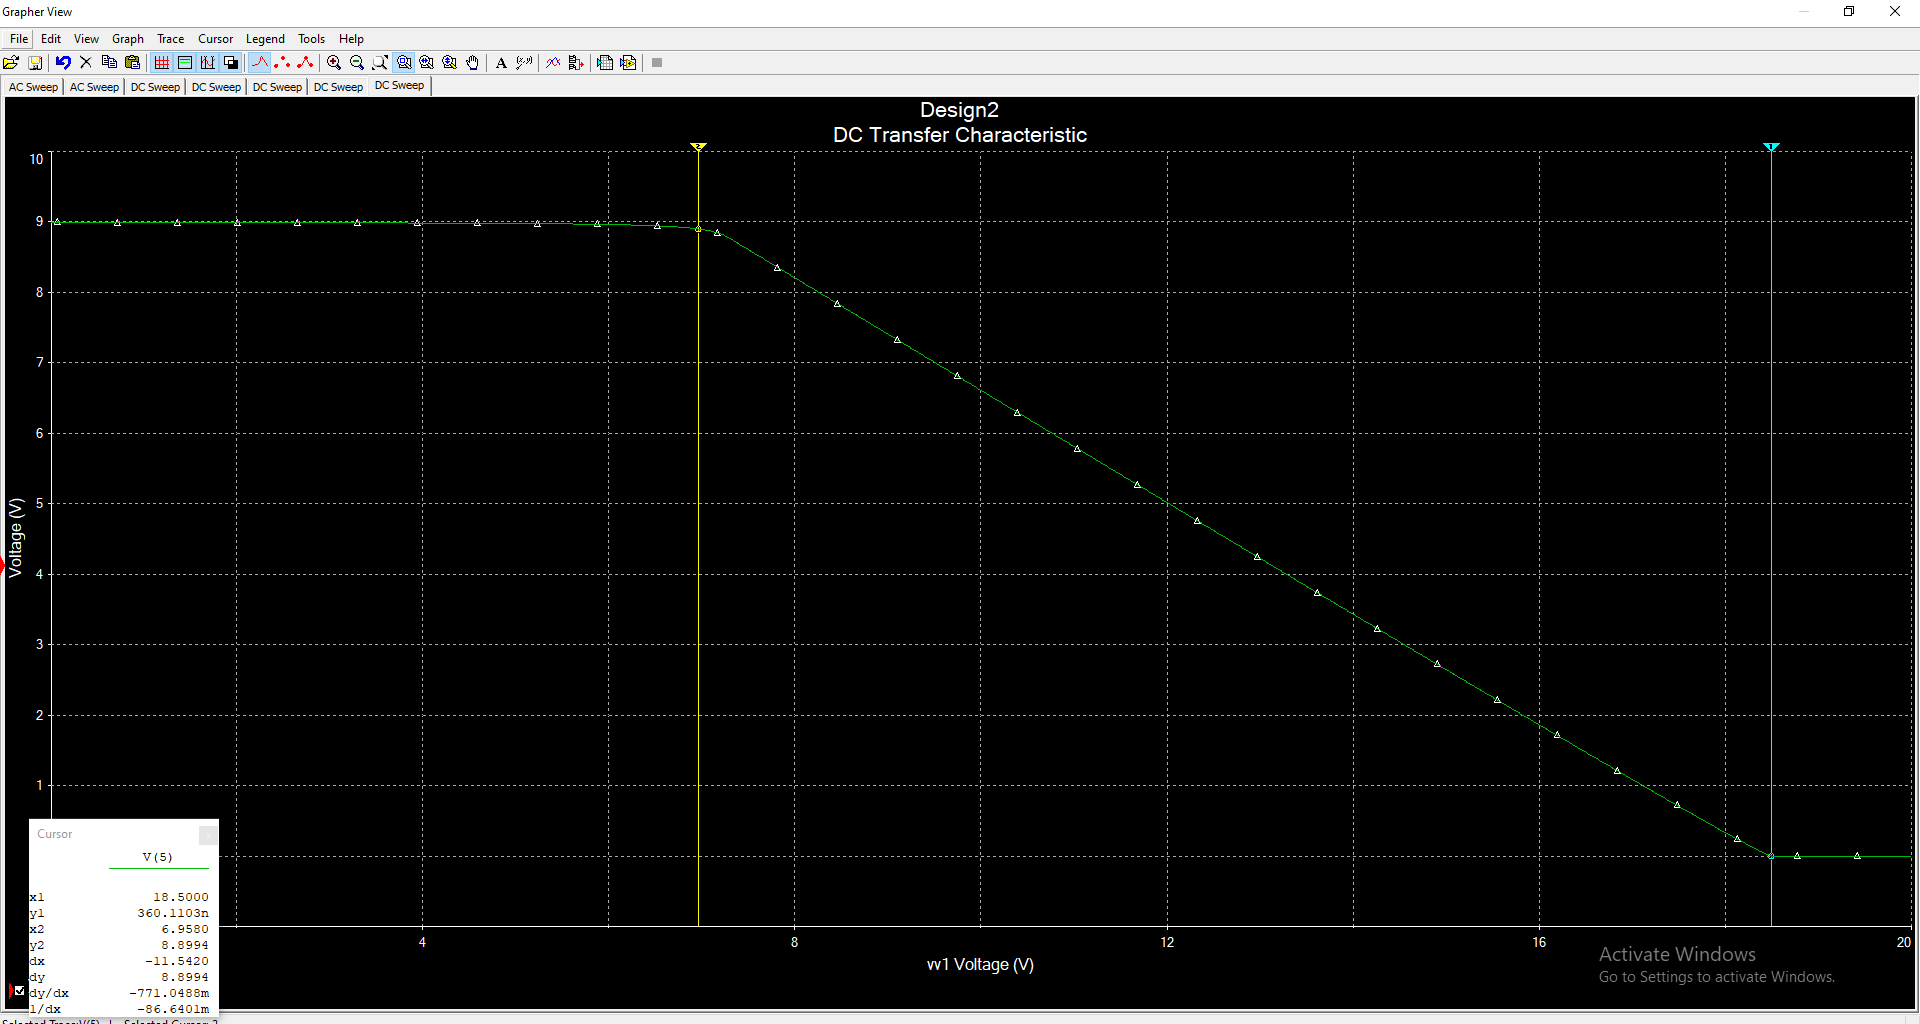
\includegraphics[width=\linewidth]{./my-chapters/my-images/Question1/Câu 1 Hình 2 a - VTC.png}
	\caption{VTC của mạch ở hình 2.}
\end{figure}

\noindent{Tìm điểm hoạt động Q:}
\[
V_{G}=V_{DD}\times\frac{R_{1}}{R_{1}+R_{2}}=20\times\frac{2.2\,\textsf{M}}{2.2\,\textsf{M}+2.2\,\textsf{M}}=10\,\textsf{V}
\]
\[
V_{DS}=V_{DD}-\left(R_{D}+R_{S}\right)\times\frac{1}{2}\times K_{p}\left(V_{GS}-V_{TP}\right)^{2}
\]
\[
V_{S}=I_{D}\times R_{S}
\]
\[
\begin{aligned}
	\Rightarrow\; V_{GS} &= V_{DD}\times\frac{R_{1}}{R_{1}+R_{2}}
	- \frac{1}{2}\times K_{p}\left(V_{GS}-V_{TP}\right)^{2}\times R_{S} \\[6pt]
	&= 10 - \frac{1}{2}\times0.4\times22\times\left(V_{GS}-V_{TP}\right)^{2} \\[6pt]
	&= -2.781\,\textsf{V}
\end{aligned}
\]

\[
V_{DS}=V_{DD}-\left(R_{D}+R_{S}\right)\times\frac{1}{2}\times K_{p}\left(V_{GS}-V_{TP}\right)^{2}
\]
\[
\Rightarrow V_{DS}=20-40\times0.5\times0.4\times\left(2.781+1.5\right)^{2}=-6.87\,\textsf{V}
\]
\[
I_{DQ}=\frac{1}{2}K_{p}\left(V_{GS}-V_{TP}\right)^{2}
\]
\[
\Rightarrow I_{DQ}=\frac{1}{2}\times0.4\times\left(-2.871+1.5\right)^{2}=0.328\,\textsf{mA}
\]

$\Rightarrow$ \finalresult{\left(I_{DQ},V_{DS}\right)=\left(0.328\,\textsf{mA},\,-6.87\,\textsf{V}\right)}.

Kiểm tra kết quả

\begin{figure}[H]
	\centering
	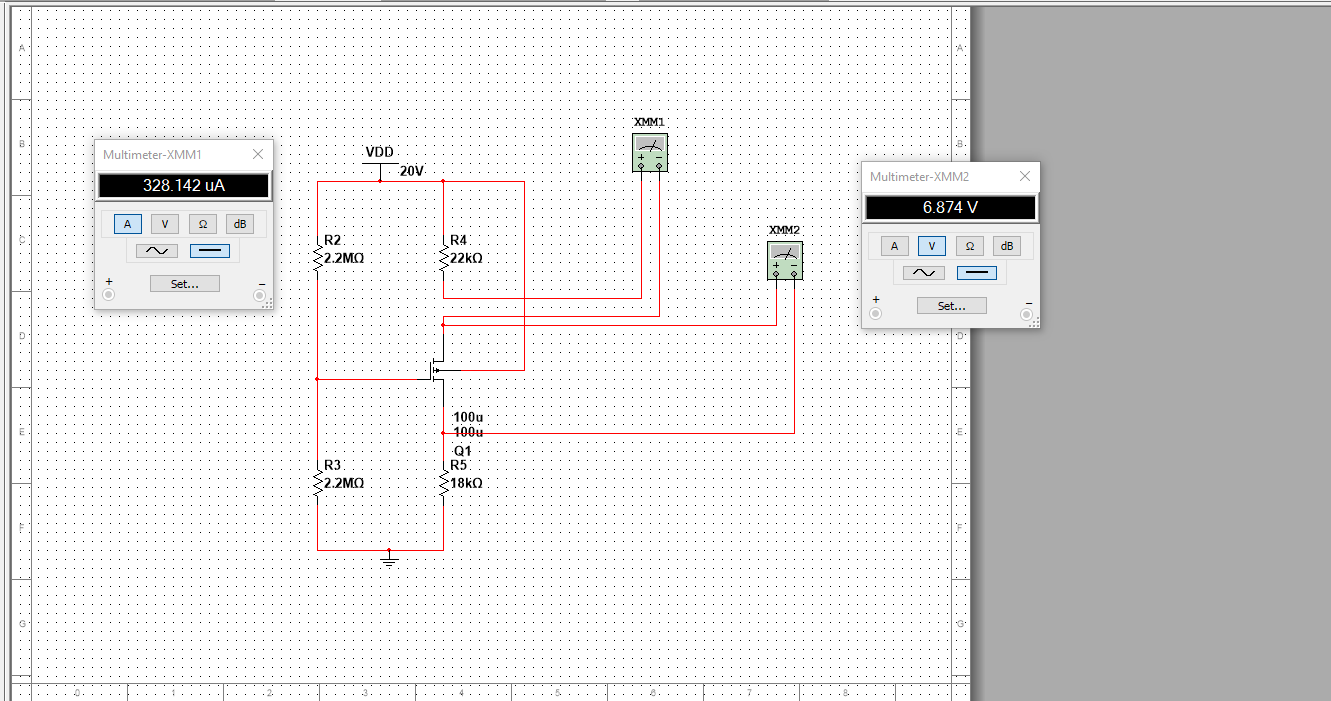
\includegraphics[width=\linewidth]{./my-chapters/my-images/Question1/Câu 1 Hình 2 a - Điểm Q.png}
\end{figure}

\answer{b2}{Tính $A_{vo}$, $G_{v}$, $R_{i}$, $R_{o}$ của mạch.}

\[
R_{i}=R_{1}\,//\,R_{2}=\frac{2.2\,\textsf{M}\times2.2\,\textsf{M}}{2.2\,\textsf{M}+2.2\,\textsf{M}}=1.1\,\textsf{M}\Omega
\]
$\Rightarrow$ \finalresult{R_{i}=1.1\,\textsf{M}\Omega}.
\[
R_{o}=R_{D}=18\,\textsf{k}\Omega
\]
$\Rightarrow$ \finalresult{R_{o}=18\,\textsf{k}\Omega}.
\[
g_{m}=\frac{2I_{DQ}}{\left|V_{GSQ}-V_{TP}\right|}=0.512\,\textsf{S}
\]
\[
A_{vo}=-g_{m}R_{D}=-9.22\,\textsf{V/V}
\]
$\Rightarrow$ \finalresult{A_{vo}=-9.22\,\textsf{V/V}}.
\[
A_{v}=A_{vo}\times\frac{R_{L}}{R_{o}+R_{L}}=-9.22\times\frac{470}{18+470}=-8.88\,\textsf{V/V}
\]
$\Rightarrow$ \finalresult{A_{v}=-8.88\,\textsf{V/V}}.
\[
G_{v}=A_{vo}\times\frac{R_{L}}{R_{o}+R_{L}}\times\frac{R_{i}}{R_{sig}+R_{i}}=-9.22\times\frac{470}{18+470}\times\frac{1.1\,\textsf{M}}{1\,\textsf{k}+1.1\,\textsf{M}}=-8.87\,\textsf{V/V}
\]
$\Rightarrow$ \finalresult{G_{v}=-8.87\,\textsf{V/V}}.

Kiểm tra kết quả

\begin{figure}[H]
	\centering
	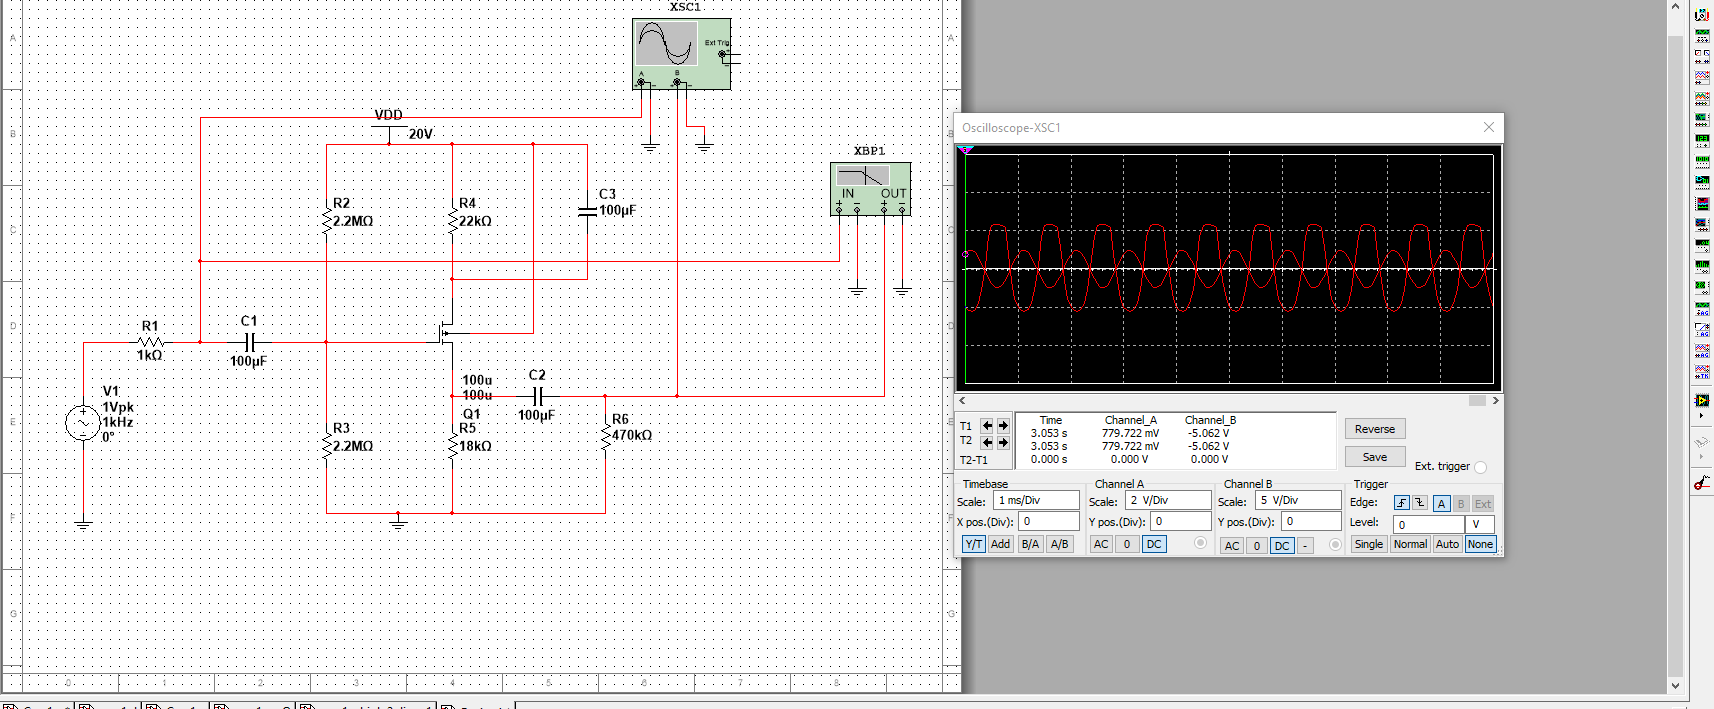
\includegraphics[width=\linewidth]{./my-chapters/my-images/Question1/Câu 1 Hình 2 b - Sóng.png}
	\caption{Dạng sóng ngõ vào và ngõ ra của mạch.}
\end{figure}

\begin{figure}[H]
	\centering
	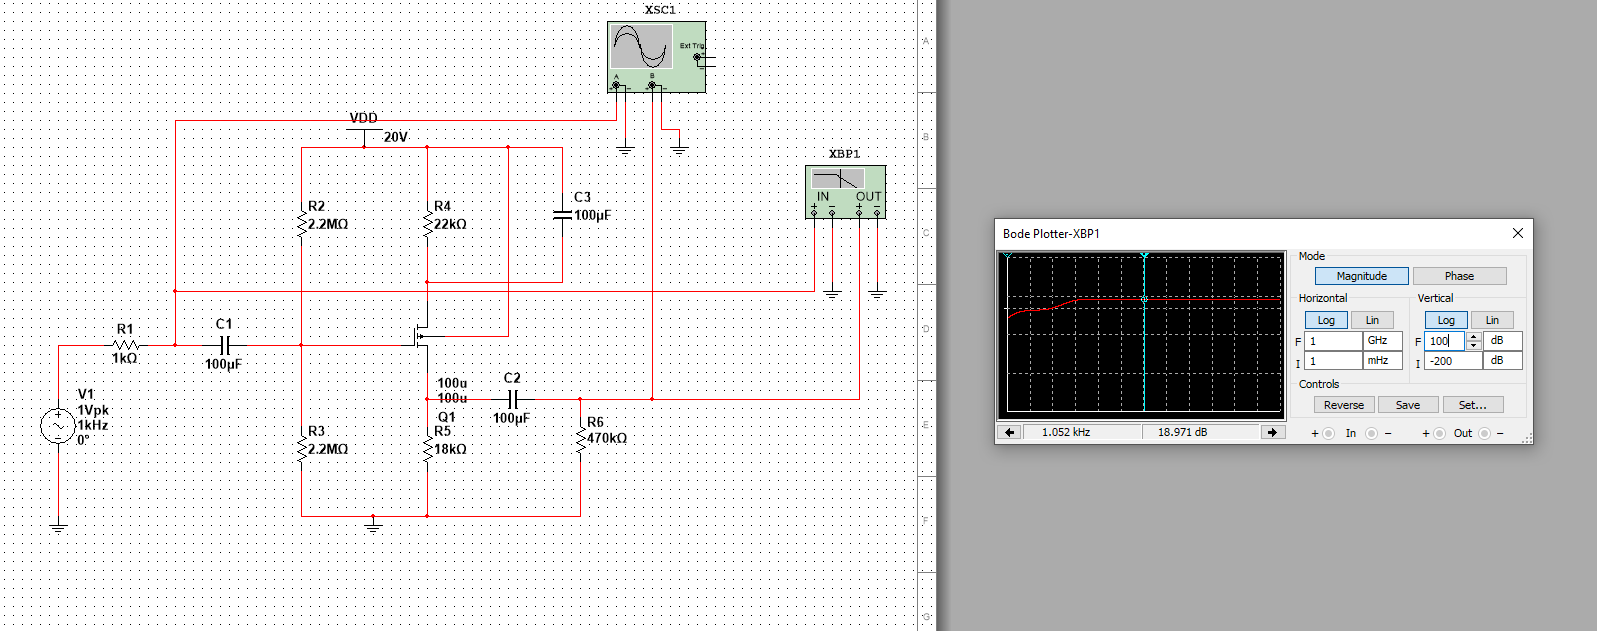
\includegraphics[width=\linewidth]{./my-chapters/my-images/Question1/Câu 1 Hình 2 b - Av.png}
	\caption{Đo $A_{v} = 18.971\, dB \approx 8.8828$.}
\end{figure}

\begin{figure}[H]
	\centering
	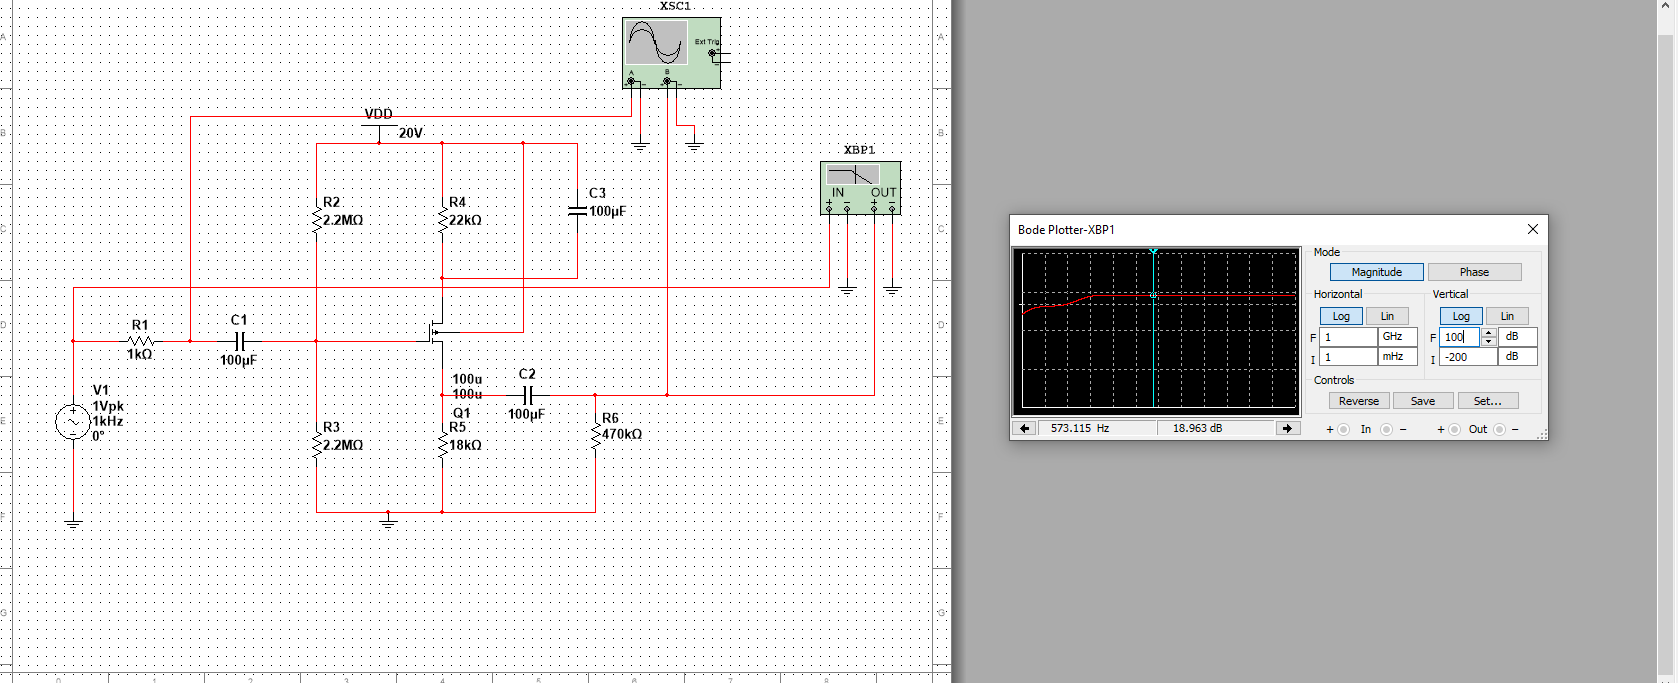
\includegraphics[width=\linewidth]{./my-chapters/my-images/Question1/Câu 1 Hình 2 b - Gv.png}
	\caption{Đo $G_{v} = 18.963\,dB \approx 8.8746$.}
\end{figure}

\answer{c2}{Tìm biên độ lớn nhất của $V_{m}$ để sóng ngõ ra không méo dạng.}

%Từ VTC, ta nhận thấy:
%\[
%{a_{v_{ds}}}_{\text{Max}}=5.36\,\textsf{V}
%\Rightarrow {a_{v_{gs}}}_{\text{Max}}=\frac{{a_{v_{ds}}}_{\text{Max}}}{\left|A_{v}\right|}=\frac{5.36}{8.88}=0.603\,\textsf{V}
%\]
%$\Rightarrow$ \finalresult{{a_{v_{gs}}}_{\text{Max}}=0.603\,\textsf{V}}.
Xét điểm $Q$ là: $\left( I_{DQ}\textsf{, } V_{DS}\right) = \left( 0.328\,\textsf{mA, } -6.87\,\textsf{V}\right)$
\[ V_{DS} = V_{DD} - \left( R_{D} + R_{S} \right) I_{DQ}\]
\[ \Rightarrow V_{DS} = 20 - 40\,\textsf{k}\times I_{DQ}\]
\[ \tan (\alpha) = \dfrac{1}{R_{D} // R_{3}} = \dfrac{1}{17\,\textsf{k}}\]
\[ \Rightarrow V_{o_{max}} = \dfrac{I_{DQ}}{\tan(\alpha)} = 5.576\,\textsf{V}\]
$\Rightarrow$ \finalresult{V_{sig_{max}} = \dfrac{V_{o_{max}}}{G_{v}\bigg|_{f=500\,\textsf{Hz}}} = 0.63\,\textsf{V}}.


\begin{figure}[H]
	\centering
	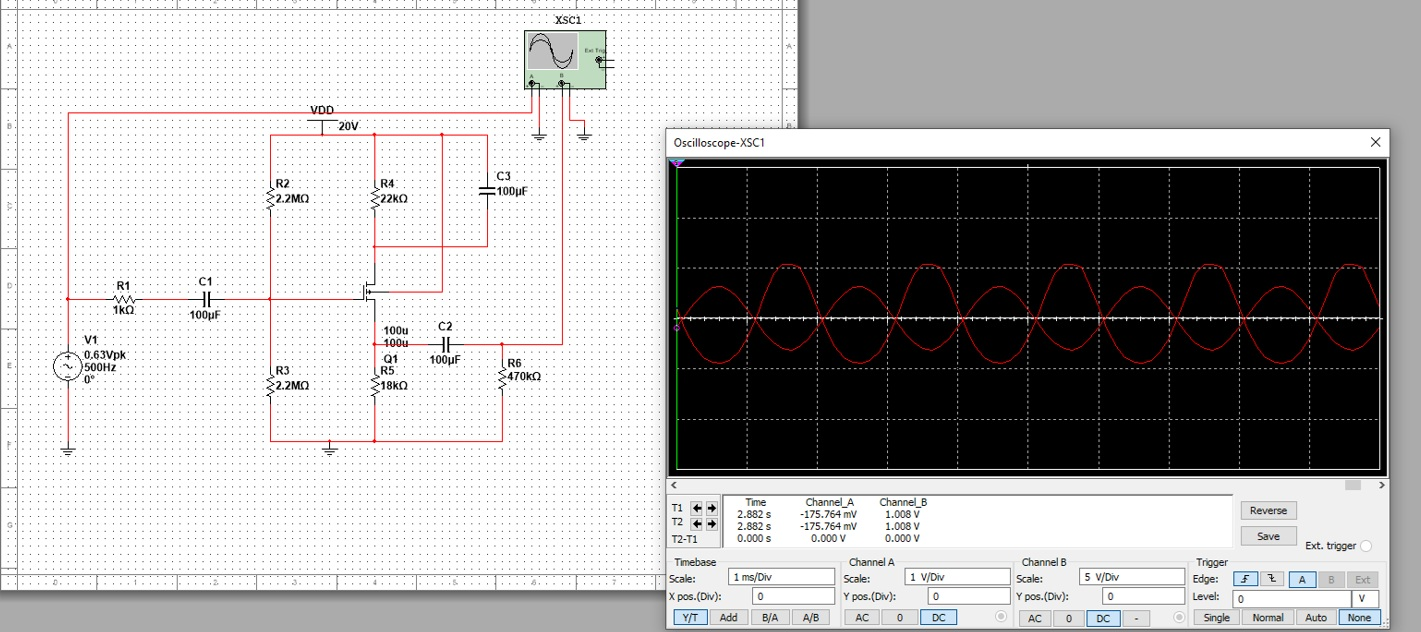
\includegraphics[width=\linewidth]{./my-chapters/my-images/Question1/c_3.jpg}
	\caption{Ngõ ra chưa bị méo dạng.}
\end{figure}
\begin{figure}[H]
	\centering
	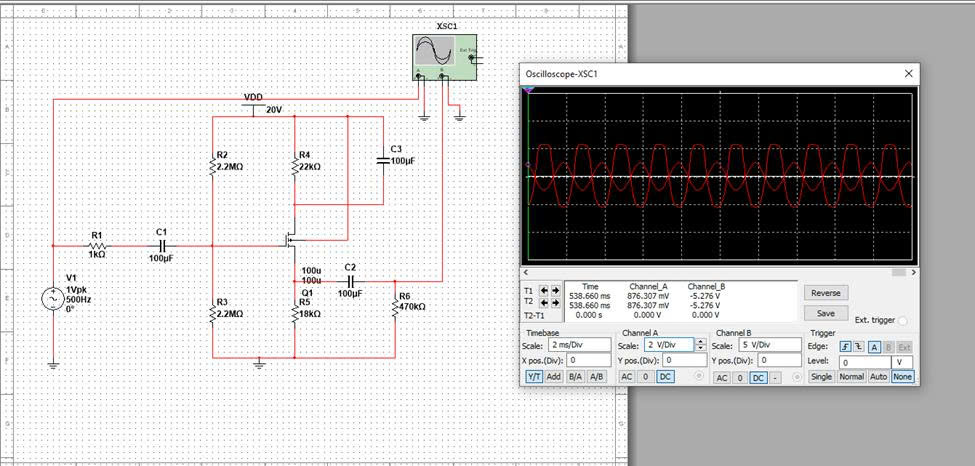
\includegraphics[width=\linewidth]{./my-chapters/my-images/Question1/c_4.jpg}
	\caption{Ngõ ra bị méo dạng.}
\end{figure}

\answer{d2}{Lựa chọn các tụ $C_{1}$, $C_{2}$, $C_{3}$ để mạch có $f_{L}=100\,\textsf{Hz}$.}

\begin{itemize}[label=-]
	\item Xét ảnh hưởng tụ $C_{1}$: 
	\[
	R_{C_{1}}=R_{sig}+R_{in}
	\Longrightarrow \omega_{p_{1}}=\frac{1}{C_{1}\left(R_{sig}+R_{in}\right)}
	\]
	
	\item Xét ảnh hưởng tụ $C_{2}$: 
	\[
	R_{C_{2}}=R_{L}+R_{D}
	\Longrightarrow \omega_{p_{2}}=\frac{1}{C_{2}\left(R_{L}+R_{D}\right)}
	\]
	
	\item Xét ảnh hưởng tụ $C_{3}$: 
	\[
	R_{C_{3}}=R_{S}\,//\,\frac{1}{g_{m}}
	\Longrightarrow \omega_{p_{3}}=\frac{1}{C_{3}\left(R_{S}\,//\,\frac{1}{g_{m}}\right)}
	\]
\end{itemize}

Theo phương pháp \textbf{cực tần số trội (dominant pole)}, chọn $C_{1}$ làm cực trội có giá trị $100\,\textsf{Hz}$, 
$C_{2}$ và $C_{3}$ tạo ra các cực ở tần số $10\,\textsf{Hz}$.  
Như vậy, tần số cắt của mạch là:
\[
f_{L}=\sqrt{f_{C_{1}}^{2}+f_{C_{2}}^{2}+f_{C_{3}}^{2}}
\]

\textbf{Lựa chọn các tụ $C_{1}$, $C_{2}$, $C_{3}$:}
\[
C_{1}=\frac{1}{2\pi\times100\times\left(1\,\textsf{k}+1.1\,\textsf{M}\right)}=1.44\,\textsf{nF}
\]
\[
C_{2}=\frac{1}{2\pi\times10\times(470\,\textsf{k}+18\,\textsf{k})}=32.6\,\textsf{nF}
\]
\[
C_{3}=\frac{1}{2\pi\times10\times\left(22\,\textsf{k}\,//\,\frac{1}{0.512\,\textsf{mS}}\right)}=8.87\,\mu\textsf{F}
\]

$\Rightarrow$ \finalresult{C_{1}=1.44\,\textsf{nF}}, \finalresult{C_{2}=32.6\,\textsf{nF}}, \finalresult{C_{3}=8.87\,\mu\textsf{F}}.

Kiểm tra kết quả

\begin{figure}[H]
	\centering
	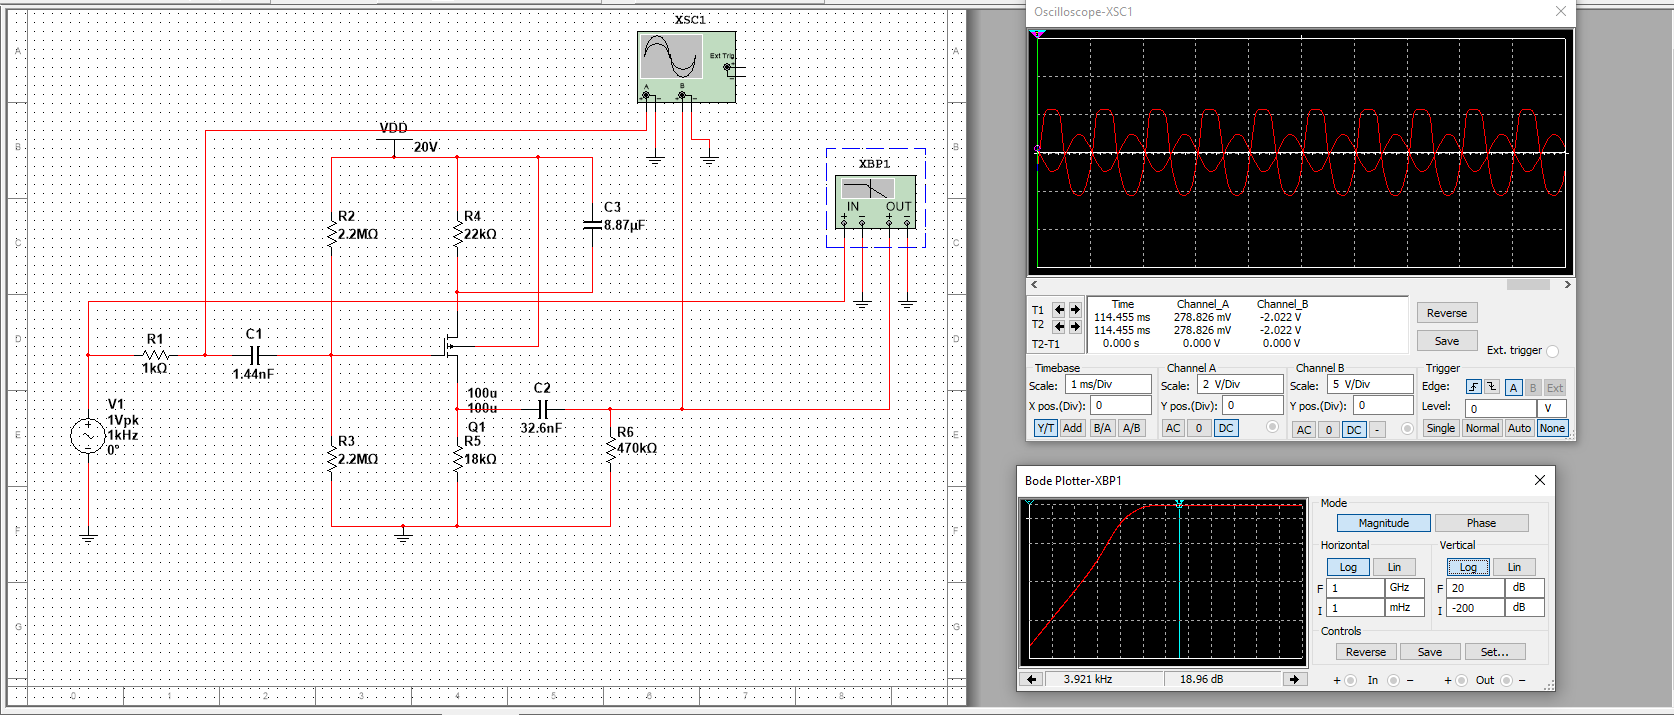
\includegraphics[width=\linewidth]{./my-chapters/my-images/Question1/Câu 1 Hình 2 d.png}
\end{figure}
